\documentclass[pdflatex,sn-mathphys-num]{sn-jnl}
\usepackage{graphicx}
\usepackage{amsmath,amssymb}
\usepackage{booktabs}
\usepackage{xcolor}
\graphicspath{{figures/}}
\renewcommand{\thesection}{S\arabic{section}}
\renewcommand{\thetable}{S\arabic{table}}
\renewcommand{\thefigure}{S\arabic{figure}}
\renewcommand{\theequation}{S\arabic{equation}}
\begin{document}
\title[Online Resource 1]{Online Resource 1: Supplementary information for ``Evidence Coverage and the Cost of False Isolation: Verifying Malicious Beacon Nodes in Mobile Ad Hoc Networks''}
\author*[1]{\fnm{Amruth} \sur{V}}\email{amruthv020@gmail.com}
\author[1]{\fnm{Devaraj} \sur{Verma C}}
\affil*[1]{\orgdiv{Department of Computer Science and Engineering}, \orgname{JAIN (Deemed-to-be University)}, \orgaddress{\city{Bengaluru}, \postcode{562112}, \state{Karnataka}, \country{India}}}
\abstract{This file holds supporting results for the main article: the per-level tables of the two attack-intensity sweeps, figures that plot results tabulated in the main text, and four secondary analyses (sensitivity to evidence orientation, localisation error, mechanism cost and the aggregation ablation). Section, table, figure and equation numbers carry the prefix S; equation numbers without it refer to the main text. The main argument can be followed without this file.}
\maketitle

\section{Attack-intensity sweep tables}
\label{sec:s1}

Tables~\ref{tab:sweep} and~\ref{tab:sweep2} give, for each intensity level of
the two sweeps in Section~6.4 of the main text, the number of seeds in which
each evidence configuration confirmed the attacker and the false confirmations
of honest beacons. Fig.~2 of the main text plots them.

\begin{table}[!t]
\caption{Primary sweep: attacker confirmed (of 10 seeds). Displacement is the
measured mean over the attacker's beacons after onset; below 45\,m it equals
the nominal $f\delta/2$ because the field boundary never clamps the offset.
Drop probability is $0.3f$. OR is the disjunctive rule over the
two single-evidence branches. FP counts honest beacons confirmed, of 20
node-seeds.}
\label{tab:sweep}
\centering
\small
\setlength{\tabcolsep}{4pt}
\begin{tabular}{@{}rrrrrrrr@{}}
\toprule
$f$ & Displ.\ (m) & Drop & Beh. & Loc. & OR & Fused & FP (OR / fused) \\
\midrule
0.025 & 3.75 & 0.0075 & 0 & 1 & 1 & 0 & 3 / 3 \\
0.05 & 7.5 & 0.015 & 3 & 0 & 3 & 3 & 5 / 4 \\
0.075 & 11.25 & 0.0225 & 6 & 0 & 6 & \textbf{3} & 1 / 1 \\
0.10 & 15.0 & 0.03 & 8 & 0 & 8 & \textbf{7} & 5 / 4 \\
0.15 & 22.5 & 0.045 & 10 & 0 & 10 & 10 & 5 / 5 \\
0.20 & 30.0 & 0.06 & 10 & 2 & 10 & 10 & 4 / 1 \\
0.30 & 45.0 & 0.09 & 10 & 9 & 10 & 10 & 4 / 4 \\
0.40 & 60.0 & 0.12 & 10 & 10 & 10 & 10 & 2 / 2 \\
0.50 & 74.9 & 0.15 & 10 & 10 & 10 & 10 & 3 / 2 \\
0.70 & 104.5 & 0.21 & 10 & 10 & 10 & 10 & 3 / 1 \\
1.00 & 147.1 & 0.30 & 10 & 10 & 10 & 10 & 3 / 3 \\
\bottomrule
\end{tabular}
\end{table}

\begin{table}[!t]
\caption{Second pairing: attacker confirmed (of 10 seeds) with drop probability
$0.15f$, half the rate of Table~\ref{tab:sweep}, at the same displacement.}
\label{tab:sweep2}
\centering
\small
\setlength{\tabcolsep}{4pt}
\begin{tabular}{@{}rrrrrrrr@{}}
\toprule
$f$ & Displ.\ (m) & Drop & Beh. & Loc. & OR & Fused & FP (OR / fused) \\
\midrule
0.10 & 15.0 & 0.015 & 3 & 0 & 3 & 3 & 5 / 4 \\
0.15 & 22.5 & 0.0225 & 6 & 1 & 6 & \textbf{7} & 1 / 1 \\
0.20 & 30.0 & 0.03 & 8 & 0 & 8 & 8 & 5 / 4 \\
0.30 & 45.0 & 0.045 & 10 & 10 & 10 & 10 & 5 / 5 \\
0.40 & 60.0 & 0.06 & 10 & 10 & 10 & 10 & 4 / 1 \\
0.50 & 74.9 & 0.075 & 10 & 10 & 10 & 10 & 2 / 2 \\
0.70 & 104.4 & 0.105 & 10 & 10 & 10 & 10 & 3 / 2 \\
1.00 & 147.1 & 0.15 & 10 & 10 & 10 & 10 & 3 / 2 \\
\bottomrule
\end{tabular}
\end{table}

\section{Supplementary figures}
\label{sec:s2}

Figs.~\ref{fig:coverage}--\ref{fig:shadow} plot results whose values are
tabulated or stated in the main text: attacker confirmation by evidence
configuration (Table~6), delivered throughput by scenario (Section~6.1), the
time of first isolation and the throughput recovery ratio by policy
(Section~6.6), false isolation by policy (Table~9) and the effect of shadowing
(Table~11).

\begin{figure}[!t]
\centering
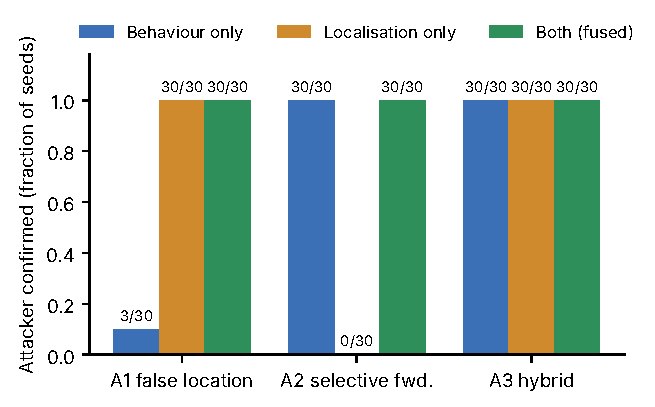
\includegraphics[width=0.78\textwidth]{fig2_coverage}
\caption{Evidence coverage over 30 seeds. Each single-evidence branch is
blind to the attack that produces no signature in its class; the three
behavioural confirmations of the A1 attacker occur at a lower rate than the
same branch confirms honest beacons.}
\label{fig:coverage}
\end{figure}

\begin{figure}[!t]
\centering
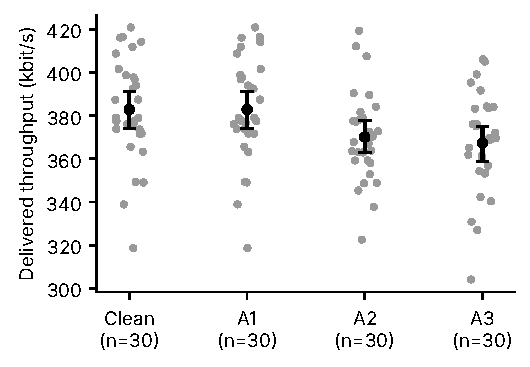
\includegraphics[width=0.6\textwidth]{fig3_throughput}
\caption{Delivered throughput by scenario, 30 seeds, with bootstrap 95\%
intervals of the mean. A1 and the clean network produce identical throughput
in every seed: the false-location attack has no packet-level footprint.}
\label{fig:tput}
\end{figure}

\begin{figure}[!t]
\centering
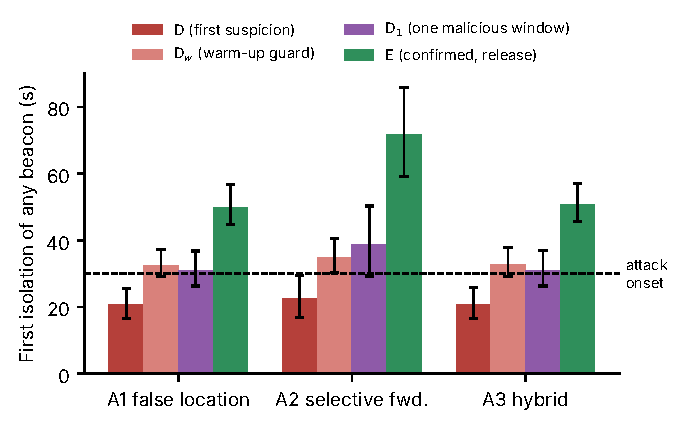
\includegraphics[width=0.78\textwidth]{fig5_first_isolation}
\caption{First isolation of any monitored beacon by policy, 30 seeds, with
bootstrap 95\% intervals. Policy D typically fires before the attack begins, so
what it first removes cannot be the attacker; D$_w$ and D$_1$ fire just after
onset, and E fires at onset plus detection latency.}
\label{fig:firstiso}
\end{figure}

\begin{figure}[!t]
\centering
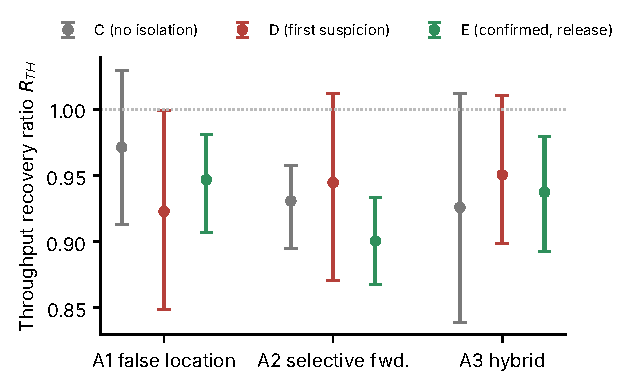
\includegraphics[width=0.68\textwidth]{fig6_recovery}
\caption{Throughput recovery ratio $R_{TH}$ in the enforced runs, five seeds,
with bootstrap 95\% intervals. The intervals exceed every between-policy
difference, so we claim no throughput advantage for any policy.}
\label{fig:recovery}
\end{figure}

\begin{figure}[!t]
\centering
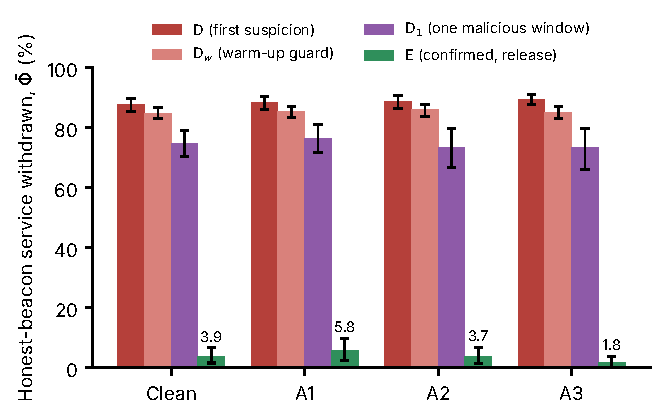
\includegraphics[width=0.8\textwidth]{fig8_phi}
\caption{Fraction of honest-beacon service withdrawn, $\bar\Phi$, by policy and
network, 30 seeds, with bootstrap 95\% intervals. Every immediate policy
withdraws 73--90\% of honest service; confirmation-gated isolation (E)
withdraws 2--6\%.}
\label{fig:phi}
\end{figure}

\begin{figure}[!t]
\centering
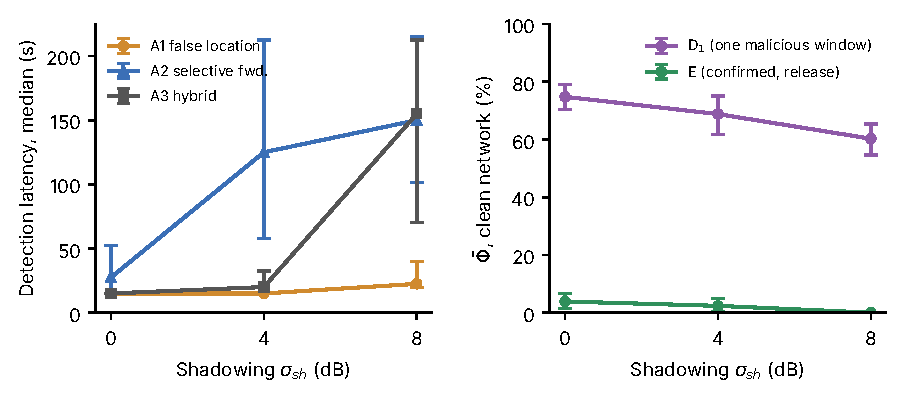
\includegraphics[width=\textwidth]{fig10_shadowing}
\caption{Effect of log-normal shadowing. Left: median detection latency, with interquartile range, rises sharply
for attacks seen through forwarding behaviour. Right: false isolation on the
clean network stays low for policy E and high for D$_1$.}
\label{fig:shadow}
\end{figure}

\clearpage


\section{Sensitivity to evidence orientation}
\label{sec:orientation}

The sign convention of Eq.~(7) of the main text deserves its own analysis, because
getting it wrong produces a detector that passes the tests most papers run and
fails the one they do not. The transform Eq.~(11) of the main text is even, but fusion
happens before $\phi$, so it is the summed statistic that is folded, not the
individual branches.

Suppose the two statistics were summed without orientation, for a beacon whose
behavioural anomaly reaches $|z_B| = 3$ and whose localisation anomaly reaches
$z_L = 3$ at full intensity, with equal weights. Under A1, $z_B \approx 0$ and
the misoriented fusion gives $Z = +2.12$, hence $T^D = 0.10$: confirmed. Under
A2, $z_L \approx 0$ and $Z = -2.12$, which because $\phi$ is even also gives
$T^D = 0.10$: confirmed. Both single-axis attacks are caught. Under a hybrid
attack at half intensity, however, $z_B \approx -1.5$ and $z_L \approx +1.5$,
and
\begin{equation}
\label{eq:cancel}
Z = \frac{(-1.5) + (+1.5)}{\sqrt2} = 0, \qquad T^D = \phi(0) = 1.0.
\end{equation}
The attacker's two misbehaviours cancel exactly, and a node misbehaving on both
axes receives perfect trust. A detector with this defect is blind to hybrid
attacks in proportion to how evenly the attacker balances the two axes, and an
adversary aware of the defect could balance them deliberately. With
Eq.~(7) of the main text applied, the same attacker gives
$Z = \bigl((+1.5) + (+1.5)\bigr)/\sqrt2 = 2.12$, recovering the full-intensity
single-axis statistic from two half-intensity observations.


\section{Localisation error}
\label{sec:locerr}

Throughput is uninformative for A1, since the attack has no packet-level
footprint. The service A1 degrades is localisation, so we report the
displacement between the position a beacon advertises and its true position,
which is the error a consumer of the localisation service inherits
(Table~\ref{tab:locerr}).

\begin{table}[!t]
\caption{Localisation error in metres, means across five seeds of the original
campaign. ``Attacker'' covers receptions from the compromised beacon; ``all''
covers every monitored beacon, of which two of three are honest.}
\label{tab:locerr}
\centering
\footnotesize
\begin{tabular}{@{}llrrrr@{}}
\toprule
Scenario & Scope & RMSE & MAE & Median & P95 \\
\midrule
Clean & all & 0.05 & 0.02 & 0.00 & 0.06 \\
A1 & attacker & 267.25 & 265.42 & 271.41 & 299.23 \\
   & all & 145.27 & 78.78 & 0.01 & 288.77 \\
A2 & attacker & 0.03 & 0.01 & 0.00 & 0.05 \\
   & all & 0.04 & 0.01 & 0.00 & 0.05 \\
A3 & attacker & 146.02 & 145.81 & 145.91 & 150.01 \\
   & all & 77.88 & 41.66 & 0.01 & 150.00 \\
\bottomrule
\end{tabular}
\end{table}

The clean-network figure of 0.05\,m RMSE confirms that honest beacons advertise
their true positions to within numerical precision, so any error observed
elsewhere is attributable to the attack. A2 produces 0.04\,m, indistinguishable
from clean: A2 is a pure forwarding attack with no positional signature, exactly
as A1 is a pure positional attack with no forwarding signature. A3's attacker
error of 146.02\,m against A1's 267.25\,m confirms the half-intensity
construction. The ratio is 0.55 instead of 0.50 because clamping binds less
often at the smaller offset.

The substantive result is the ``all'' row. Under A1 the mean error across all
monitored beacons is 145.27\,m while the median is 0.01\,m. Two of three beacons
are honest and contribute essentially zero error, while the third contributes
the full displacement. A localisation consumer drawing on the affected beacon
inherits an error more than three orders of magnitude above the clean-network floor, and
averaging over honest neighbours does not conceal it, since trilateration
depends on all contributing anchors.


\section{Mechanism cost}

\begin{figure}[!t]
\centering
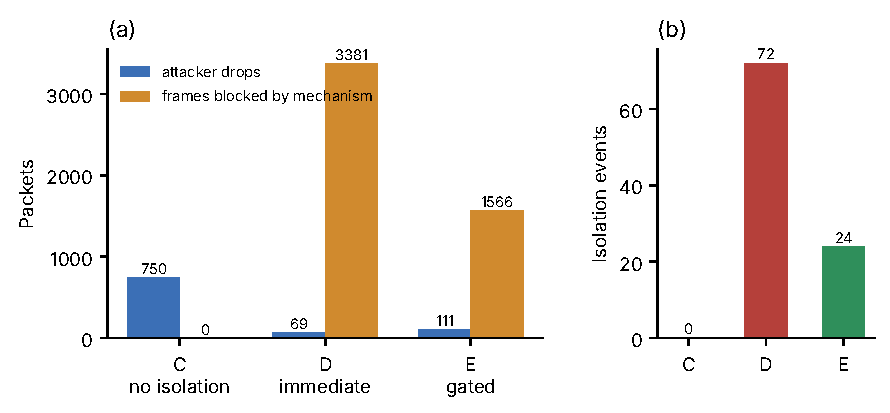
\includegraphics[width=0.8\textwidth]{fig7_mechanism}
\caption{Isolation mechanism accounting in one illustrative enforced run (A2,
seed 1), not an aggregate. Policy D suppresses more attacker drops but blocks
more than twice as many frames and performs three times as many isolation
events as policy E.}
\label{fig:mechanism}
\end{figure}

Fig.~\ref{fig:mechanism} decomposes what each policy does within a single run.
The counters were logged per run but not aggregated across the campaign, so the
figure illustrates the accounting without establishing a general magnitude.
Both policies suppress attacker drops substantially relative to the control:
from 750 packets under C to 69 under D and 111 under E. Frames blocked by the
enforcement mechanism itself differ by more than a factor of two, 3381 under D
against 1566 under E, tracking isolation-event counts of 72 and 24. The counter
separates the mechanism's benefit from its cost within a run, which aggregate
PDR does not.


\section{Aggregation ablation}
\label{sec:ablation}

\begin{table}[!t]
\caption{Aggregation ablation, original campaign. Confirmations out of 15
target-seeds per cell.}
\label{tab:ablation}
\centering
\footnotesize
\begin{tabular}{@{}lcccc@{}}
\toprule
Configuration & A1 & A2 & A3 & Clean \\
\midrule
Direct only & 6/15 & 5/15 & 6/15 & 1/15 \\
Direct + indirect & 6/15 & 5/15 & 6/15 & 1/15 \\
Direct + indirect + historical & 6/15 & 5/15 & 6/15 & 1/15 \\
\bottomrule
\end{tabular}
\par\smallskip\footnotesize
Counts include false confirmations: A1 6/15 is the attacker in five seeds plus
one honest beacon.
\end{table}

\begin{figure}[!t]
\centering
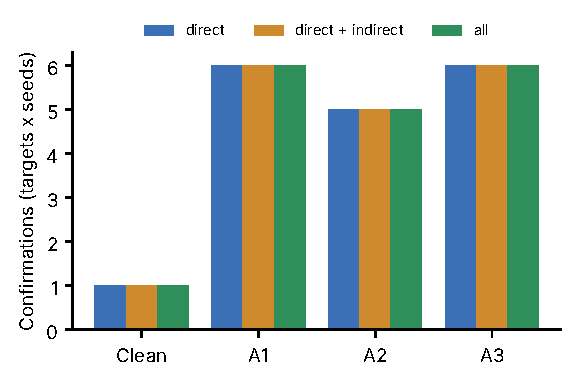
\includegraphics[width=0.62\textwidth]{fig9_ablation}
\caption{Aggregation ablation. The three configurations are identical in every
cell: adding indirect and historical trust changes no verdict.}
\label{fig:ablation}
\end{figure}

Table~\ref{tab:ablation} and Fig.~\ref{fig:ablation} report the second stage
ablated across its components. History-only is not an admissible configuration,
since $T^H$ seeds from the combined value. The three configurations are
identical in every cell. The components are not inert in the underlying
computation: on A2 seed~1, direct-only aggregation gives mean trust 0.7148
with 50 window-level confirmations, while direct plus indirect gives 0.7548
with 70. But the differences never cross the persistence gate, so no target's
final verdict changes. $T^H$ is an exponentially weighted average of combined
trust, itself dominated by direct trust, and $T^I$ a trimmed mean of peers' direct trust: both are smoothed
functions of the same underlying signal, and they would be expected to diverge
only where direct trust is noisy and observers disagree, a regime our topology
does not produce often enough to matter.



\end{document}
